\chapter{Versuchsdurchführung}

\section{Versuchsaufbau}

Folgende Hardware sollte sich in Ihrer Versuchskiste befinden. Bitte überprüfen sie dies vor Beginn des Versuches.

\begin{itemize}
    \item RespberryPi 3 mit eingesetzter microSD-Karte
    \item CC2531 Sniffer Stick
    \item cod.m ZigBee CC2652P2 Raspberry Pi Module
    \item 2 x Phillips Hue White E27
    \item 1 x Phillips Hue dimmer switch
    \item HDMI Kabel
    \item Ethernet Kabel
\end{itemize}

Ein cod.m Zigbee Modul sollte bereits auf Ihrem Raspberry montiert sein. 

In diesem Praktikumsversuch wird ein kleinen ZigBee Netzwerk errichtet. Verschiedene Funktionen des Protokolls werden getestet und aufgezeichnet.


\begin{figure}[H]
    \centering
    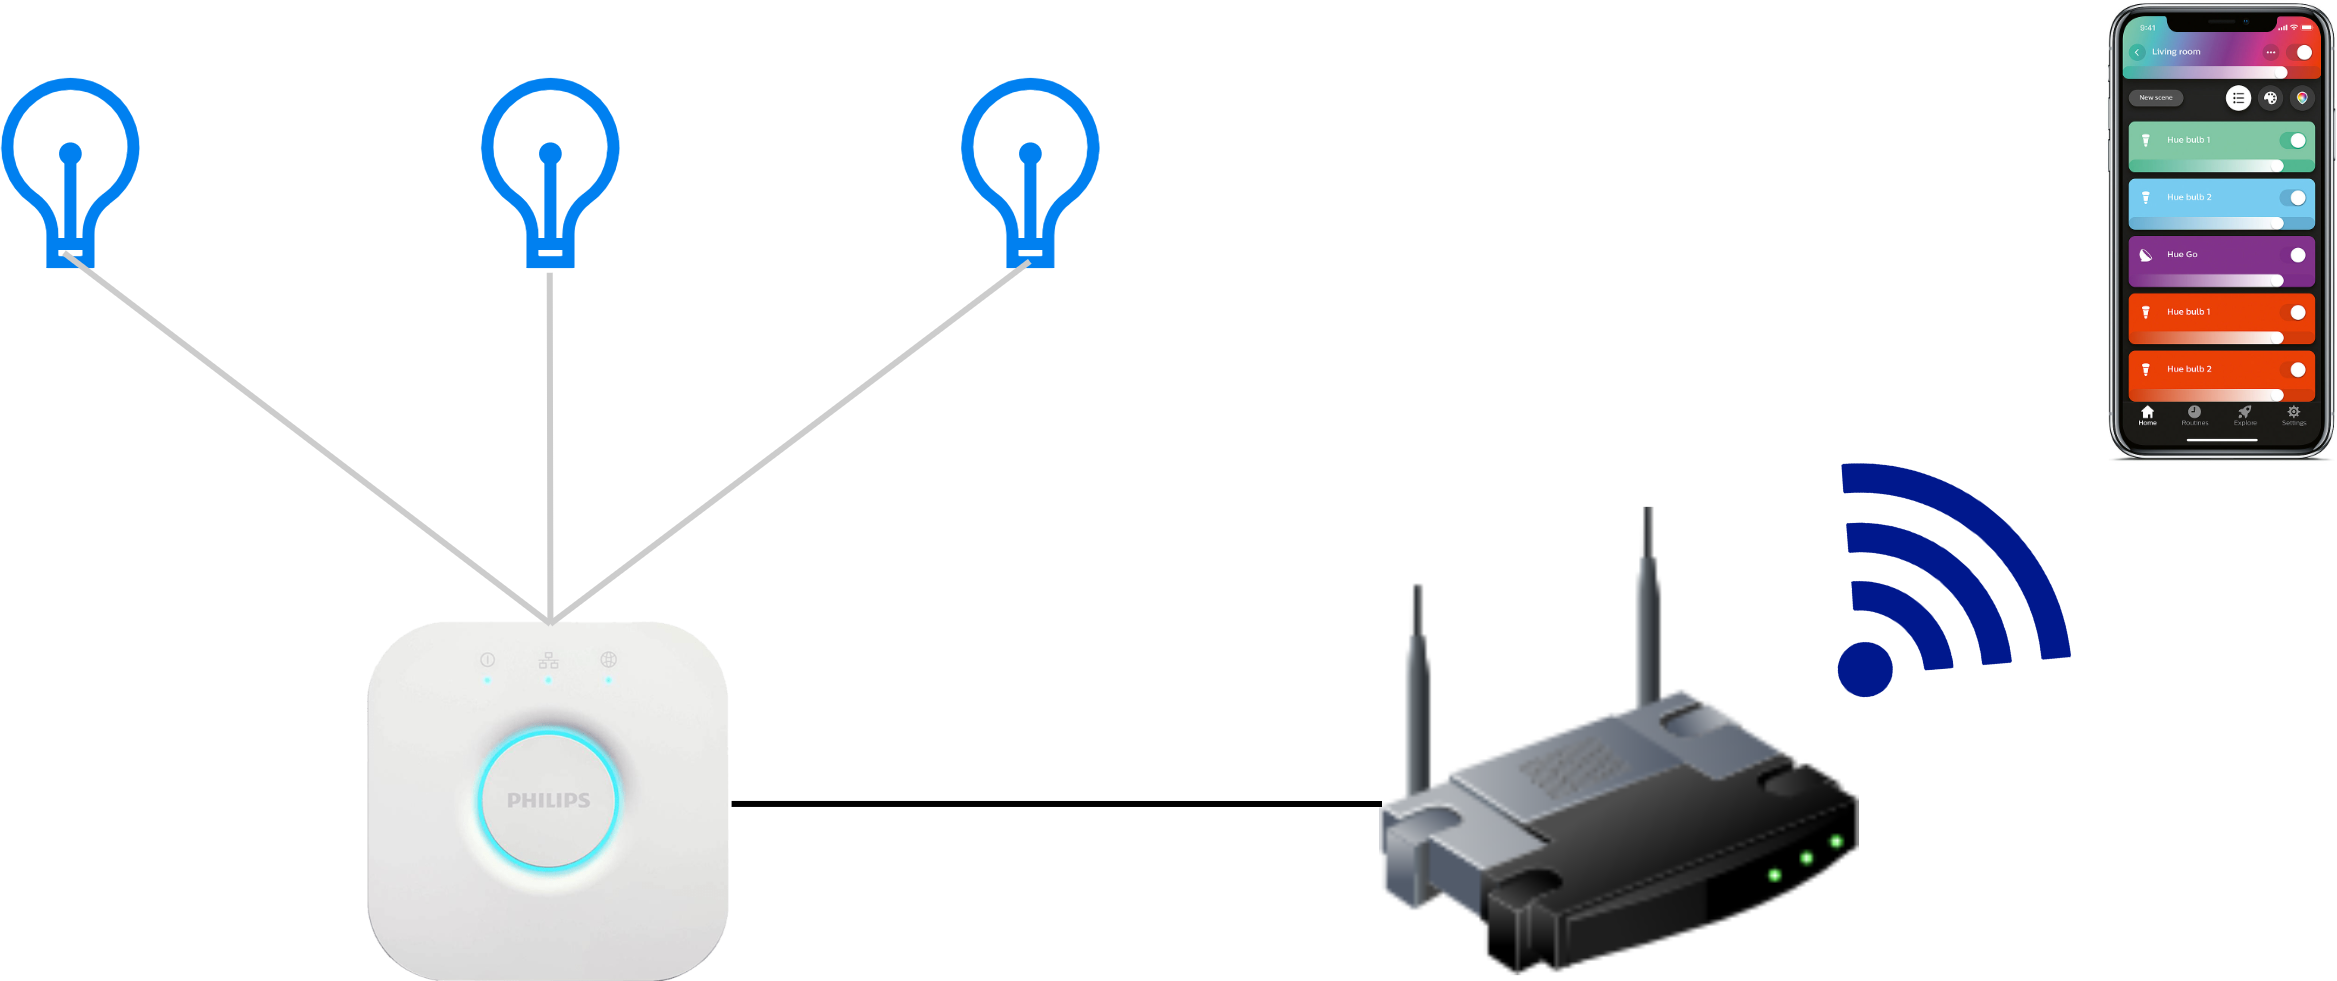
\includegraphics[width=1\textwidth]{media/zbhue.png}
    \caption{Phillips Hue}
\end{figure}
Das ZigBee Protokoll, welches in diesem Versuch untersucht wird, kommt klassischerweise in hier gezeigtem Szenario zum Einsatz.
Eine Bridge, hier von Phillips, verbindet sich per ZigBee mit Smarthome Komponenten wie Lampen. Diese Bridge fungiert als ZigBee Koordinator. 
Eine Smartphone App greift per REST-API auf die Bridge zu. Mit der App können nun die Lampen gesteuert werden.

\begin{figure}[H]
    \centering
    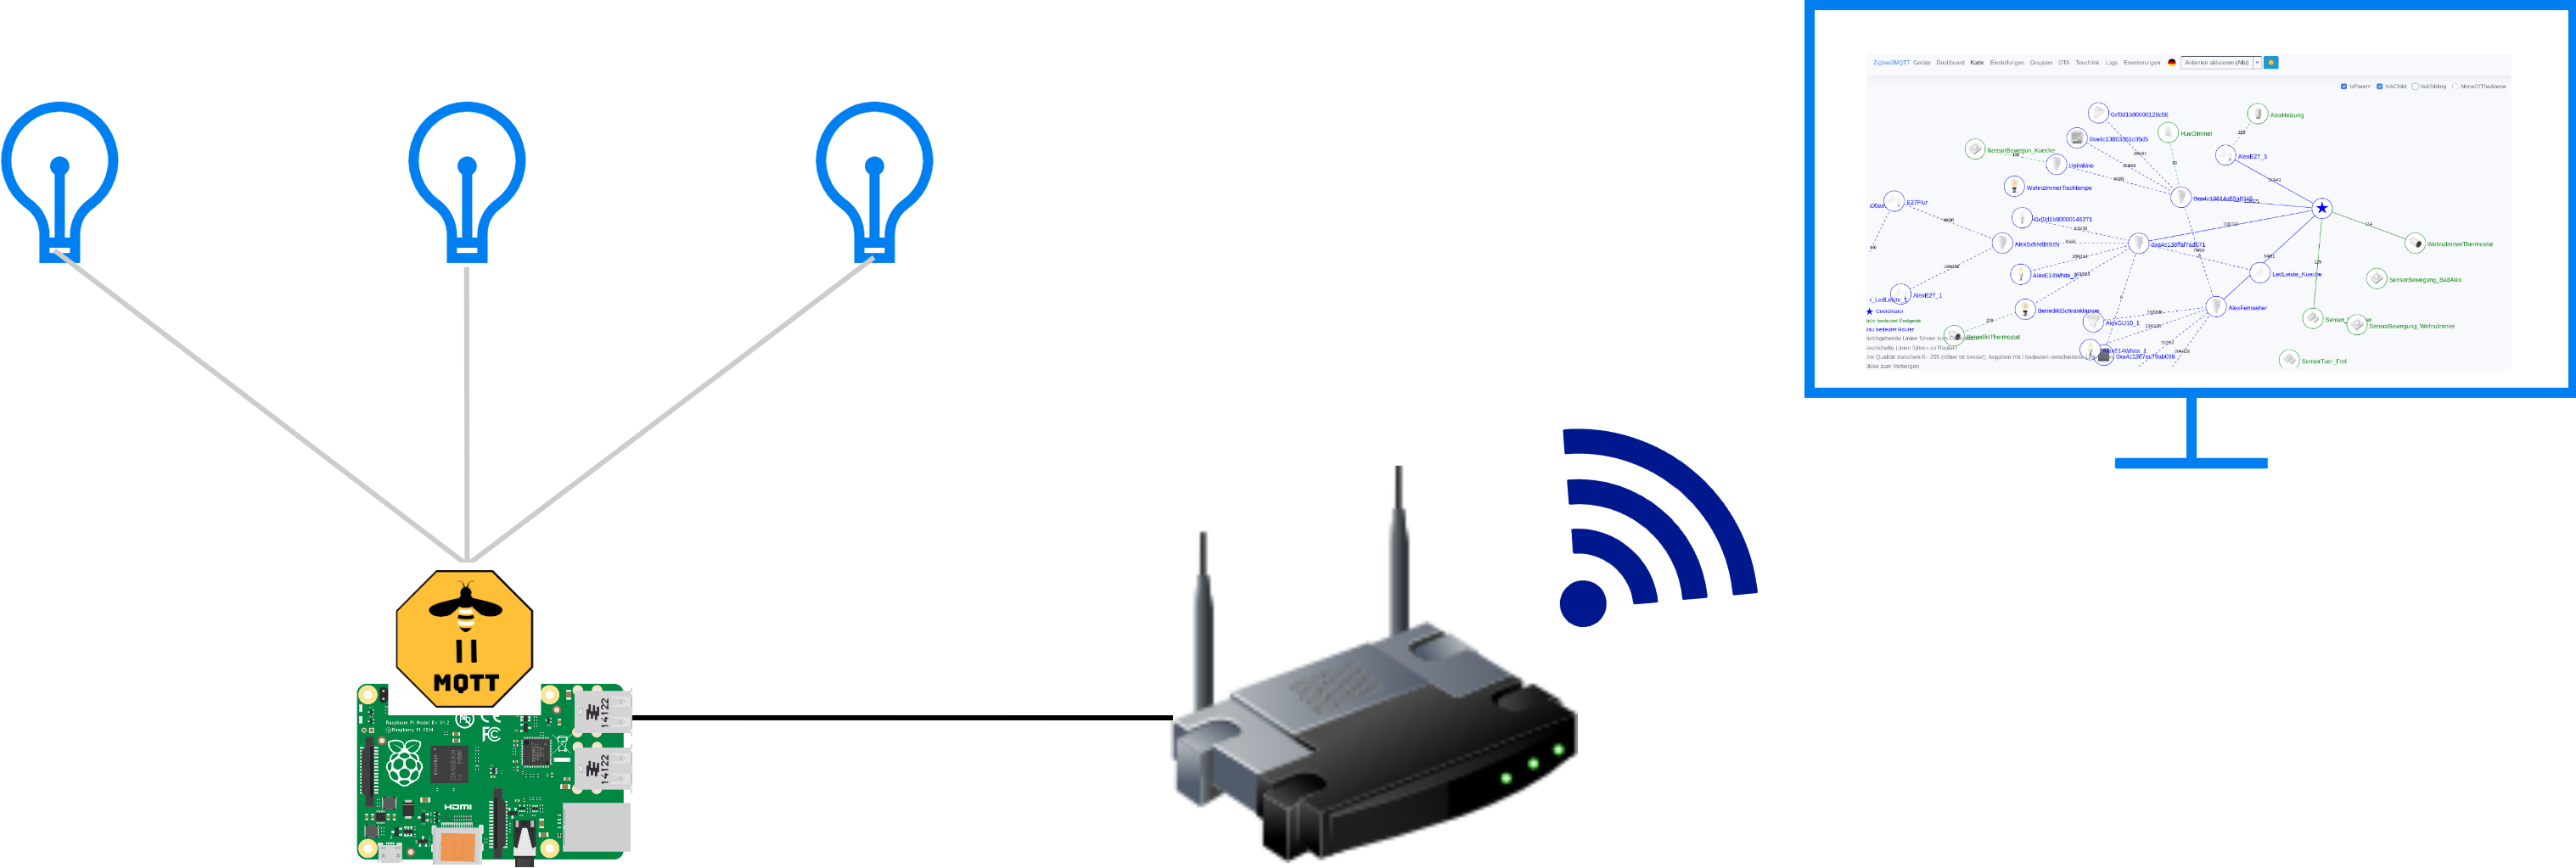
\includegraphics[width=1\textwidth]{media/zbz2m.png}
    \caption{Versuchsaufbau}
\end{figure}

In diesem Versuch wird anstelle der Phillips Bridge ein RaspberryPi als Koordinator eingesetzt. Dieser benötigt dafür das cod.m Zigbee Modul sowie eine entsprechende
Software. In dem Versuch wird zigbee2mqtt eingesetzt. Anstelle einer App wird zigbee2mqtt über ein Webinterface administriert. Dieses lässt sich wie in diesem Versuch gezeigt Lokal 
aufrufen oder aber auch nach außen verfügbar machen. 

Der RaspberryPi dient in diesem Versuch als Koordinator und Versuchs-PC zugleich. 

\section{Aufgabenstellungen}

Bitte arbeiten sie die folgenden Aufgabenstellungen durch. Fertigen sie im Anschluss einen Versuchsbericht an. Beantworten sie die anhängenden Fragen
implizit oder explizit.

\subsection{Aufgabe 1 - Vorbereitungen}

\subsubsection{Vorbereitung}
a) Schließen sie an den RaspberryPi Monitor, Tastatur, Maus sowie den Sniffer-Stick an. Durch Anschluss der
Stromversorgung startet der RaspberryPi automatisch. 

b) Starten sie den Versuch, in dem sie ein Konsolenfenster öffnen und folgenden Befehl absetzen.

\begin{lstlisting}
    > ansible-playbook ~/ZigbeeHSRM/playbooks/reset-lab.yaml -K -e "channel=<Gruppennummer>"
\end{lstlisting}

Setzen sie den gewünchten Kanal für <Gruppennummer> ein. Der Start des Labs kann einige Minuten dauern. Dieser Befehl muss nur einmal zu Beginn
des Praktikums ausgeführt werden. Bei einem Neustart des RaspberryPis startet der Versuch automatisch. Sie werden nach einem Passwort gefragt. 
Das Passwort sollte gleich dem Benutzernamen sein. Im zweifel Fragen sie Ihren Betreuer.

c) Starten sie ein Konsolenfester und überprüfen mit folgendem Befehl, ob die Container ausgeführt werden:
\begin{lstlisting}
    > docker ps
\end{lstlisting}

Es sollten 3 Container im Status \grqq Running\grqq{} sein. Sollte dies nicht der Fall sein, beispielsweiße ein periodisches Neustarten des Containers 
\grqq zigbee2mqtt\grqq{}, lesen sie die weiteren Schritte in den FAQs nach.

d) Starten sie den Webbrowser und Navigieren zu der Seite:
\begin{lstlisting}
    https://z2m.local
\end{lstlisting}

e) Starten sie Wireshark per \grqq sudo wireshark\grqq{} in einem Terminalfenster. Bei den verfügbaren Schnittstellen sollte sich eine 
\grqq TI CC2231\grqq{} Schnittstelle finden. Über das vorangestelle Zahnrad-Symbol können sie den mitzuschneidenden
 Kanal einstellen. Stellen sie den eben gewählten Zigbee Kanal ein. (Gruppennummer)

d) Setzen sie alle ZigBee Komponenten des Versuchs zurück. Dafür drücken sie auf der Rückseite der Fernbedienung die Reset Taste.
Die Phillips Hue Lampen können auschließlich per Touchlink zurückgesetzt werden. Drücken und halten sie dazu die äußeren Tasten der Fernbedienung während sie die Fernbedienung
direkt an die Lampe halten. Warten sie bis die Lampe mehrmals aufblinkt. Dies kann mehrere Versuche mit verschiedenen Fernbedienungspositionen benötigen. Schalten sie im Anschluss
die beiden Lampen wieder per Handschalter vollständig aus.

Alternativ bietet zigbee2mqtt ebenfalls eine Touchlink Funktionalität. Bringen sie dafür die Lampe direkt an den Koordinator und Scannen in dem zigbee2mqtt Webinterface nach 
Touchlink Geräten. Im Anschluss kann die Lampe hier zurückgesetzt werden. Auch hier wird das durch mehrmaliges blinken der Lampe signalisiert.

\begin{figure}[H]
    \centering
    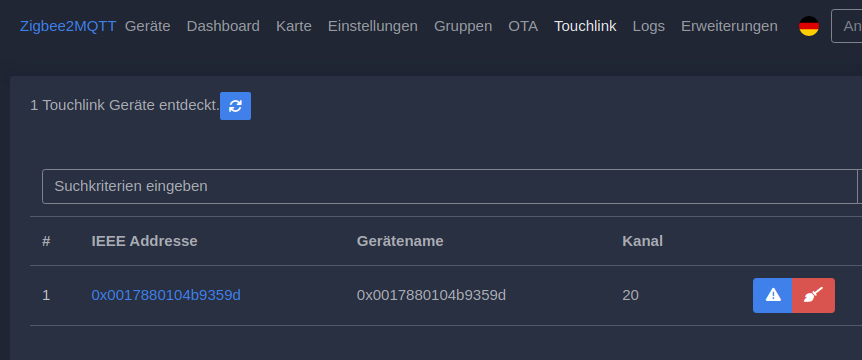
\includegraphics[width=1\textwidth]{media/z2m-touchlink.png}
    \caption{Touchlink - Lampen zurücksetzen}
\end{figure}

\begin{Hinweis}
    Alle Aufgaben sollen mit Wireshark mitgeschnitten werden. Lesen sie die Aufgabenstellung erst durch und machen sie sich den Ablauf klar. Versuchen sie das 
    Zeitfenster des Wireshark Mitschnitts kurz halten, und in dieser Zeit nur die in der Aufgabenstellung explizit beschriebenen Aktionen durchzuführen.
\end{Hinweis}

\subsection{Aufgabe 2 - Joining einer Phillips Hue Lampe}
a) Schalten sie eine der beiden Lampen ein.\\\\
b) Starten sie nun ein Wireshark Mitschnitt und erlauben anschließend in zigbee2mqtt das Anlernen von Geräten. Sobald zigbee2mqtt ein erfolgreiches Interview gemeldet hat, 
beenden sie den Capture Vorgang. Die Lampe signalisiert dies durch ein kurzes blinken ein erfolgreiches Interview.\\\\

\begin{figure}[H]
    \centering
    
\includegraphics[width=1\textwidth]{media/Z2M-Anlernen.png}
    \caption{Zigbee Anlernen aktivieren}
\end{figure}

\begin{Aufgabe}
    Speichern sie den Wireshark Capture ab als \textbf{\grqq <Gruppe>-ZigbeeLab-Aufgabe2.1\grqq{}}. \\
    Beantworten sie die Fragen in Ihrem Versuchsbericht.
\end{Aufgabe}

c) Navigieren sie nun zur Übersichtsseite der Lampe. Diese sollte ähnlich wie folgende Seite aussehen:

\begin{figure}[H]
    \centering
    \includegraphics[width=1\textwidth]{media/Z2M-Übersichtsseite.png}
    \caption{Zigbee Device Übersicht}
\end{figure}

d) Vergeben sie in der Übersichsseite der Lampe einen nutzerfreundlichen Namen. Dies geschieht über den blauen Button im unteren Teil der Übersicht.\\
e) Dimmen und schalten sie die Lampe über die Weboberfläche. Die ist unter dem Reiter \grqq Dashboard\grqq{} möglich. Starten sie einen weiteren Capture Vorgang und
schneiden einen Schaltvorgang mit.

\begin{Aufgabe}
    Speichern sie den Wireshark Capture ab als \textbf{\grqq <Gruppe>-ZigbeeLab-Aufgabe2.2\grqq{}}. \\
    Beantworten sie die Fragen in Ihrem Versuchsbericht.
\end{Aufgabe}

\subsection{Aufgabe 3 - Joining eines Gerätes über ein anderes Gerät}
Für diese Aufgabe sollte eine Lampe mit dem Koordinator verbunden sein. Die zweite Lampe wird nun über die Lampe dem Netzwerk hinzugefügt. Aus diesem Grund wird es nur der Lampe
erlaubt ein neues Gerät in das Netzwerk aufzunehmen. 

a) Schalten sie die zweite Lampe ein und starten einen Wireshark Mitschnitt.\\
b) Erlauben sie den Beitritt neuer Geräte explizit für die bereits verbundene Phillips Lampe.
Ein erfolgreiches anlernen wird auch hier in der Weboberfläche und durch ein blinken der Lampe signalisiert. 

\begin{figure}[H]
    \centering
    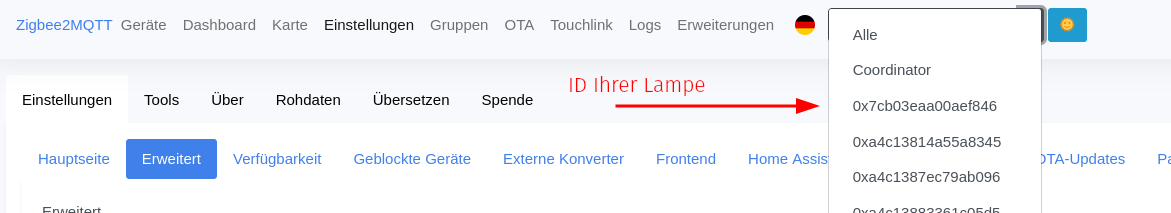
\includegraphics[width=1\textwidth]{media/Z2M-Anlernen-Lampe.png}
    \caption{Zigbee Anlernen aktivieren - nur Lampe}
\end{figure}

\begin{Aufgabe}
    Speichern sie den Wireshark Mitschnitt ab als \textbf{\grqq <Gruppe>-ZigbeeLab-Aufgabe3\grqq{}}. \\
    Beantworten sie die Fragen in Ihrem Versuchsbericht.
\end{Aufgabe}

c) Sehen sie sich die Netzwerkübersicht unter dem Reiter \grqq Karte\grqq{} an. Aktivieren sie nur den Haken \grqq isParent\grqq{} \\
d) Fügen sie die Fernbedienung Ihrem Netzwerk hinzu. Gehen sie dabei wie bisher vor. Setzen sie die Batterie in die Lampe ein und erlauben die Aufnahme neuer Geräte.

Ihre Übersichtsseite sollte wie folgt aussehen.

\begin{figure}[H]
    \centering
    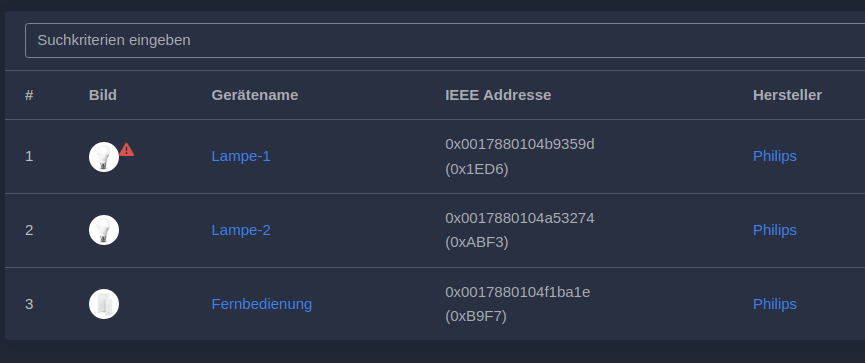
\includegraphics[width=1\textwidth]{media/z2m-ov.png}
    \caption{Zigbee2mqtt Übersichtsseite Lab}
\end{figure}


\subsection{Aufgabe 4 - Binding der Fernbedienung}

a) Navigieren sie in der Weboberfläche zu der Übersicht Ihrer Lampe. Dort finden sie einen Reiter \grqq binden\grqq{}. \\
b) Starten sie ein Wireshark Mitschnitt. Binden sie den Endpunkt der Fernbedienung mit dem Endpunkt Ihrer Fernbedienung. Binden sie die Cluster \grqq OnOff\grqq{}
und \grqq LevelCtrl\grqq{}. Betätigen sie direkt nach dem Anlegen der Bindung eine Taste auf der Fernbedienung. Zum Batteriesparen \grqq schläft\grqq{} diese 
periodisch und kann in dieser Zeit keine Bindungsanfragen annehmen. Der Hersteller geht davon aus, das die Fernbedienung gewöhnlich per Touchlink gebunden wird. 
Warten sie bis zigbee2mqtt ein erfolgreiches Binding meldet. \\



Achten sie darauf alle die gezeigten Cluster anzuwählen. Jedes Cluster wird einzeln gebunden.

c) Schalten sie nun die Lampe mit der Fernbedienung ein und aus. 

\begin{Hinweis}
    Speichern sie den Wireshark Capture ab als \textbf{\grqq <Gruppe> - ZigbeeLab - Aufgabe 4\grqq{}}. \\
    Beantworten sie die Fragen in Ihrem Versuchsbericht.
\end{Hinweis}

d) Entfernen sie im Anschluss dieses Binding. Drücken sie auch hier eine Taste der Fernbedienung damit diese geweckt wird.

\subsection{Aufgabe 5 - Gruppenbildung}

a) Navigieren sie in der Weboberfläche zu dem Reiter \grqq Groups \grqq{}. \\
b) Legen sie eine Gruppe mit dem Namen \grqq Hue-Lights-<Gruppe> \grqq{} an.\\
c) Starten sie einen Wireshark Mitschnitt. Editieren sie nun die Gruppe. Fügen sie die Endpunkte der beiden Lampen, die zum Steuern verwendet werden, der Gruppe hinzu. \\


\begin{Aufgabe}
    Speichern sie den Wireshark Capture ab als \textbf{\grqq <Gruppe> - ZigbeeLab - Aufgabe 5\grqq{}}. \\
    Beantworten sie die Fragen in Ihrem Versuchsbericht.
\end{Aufgabe}

d) Navigieren sie nun wieder zur Binding-Übersicht der Fernbedienung. Binden sie die Fernbedienung nun mit der soeben
angelegten Gruppe. Achten sie auch hier darauf eine Taste der Fernbedienung zu betätigen.\\

\begin{figure}[H]
    \centering
    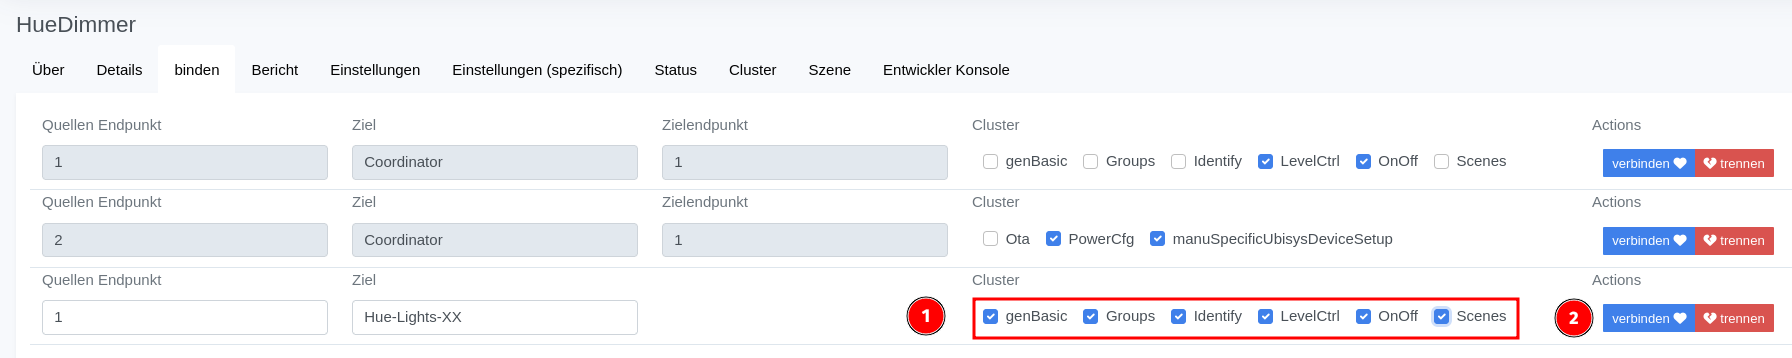
\includegraphics[width=1\textwidth]{media/Z2M-Group-Binding.png}
    \caption{Zigbee2mqtt Group Binding}
\end{figure}

e) Starten sie einen Wireshark Mitschnitt. Schalten sie die Gruppe mit der Fernbedienung ein und aus.

\begin{Aufgabe}
    Speichern sie den Wireshark Capture ab als \textbf{\grqq <Gruppe> - ZigbeeLab - Aufgabe 5.1\grqq{}}. \\
    Beantworten sie die Fragen in Ihrem Versuchsbericht.
\end{Aufgabe}

\subsection{Fragen}
\subsubsection{Aufgabe 2}
\begin{Fragen}
    1. Untersuchen sie den \textbf{Beacon-Request}\\
    - Erläutern sie den Frametype und den Command Identifier.\\ 
    - Erläutern die Ziel- und Quelladdresse und was sie daraus erschließen können.\\
    Hinweis: Wireshark Filter: \verb|frame.protocols == "wpan"|\\

    2. Wie teilt der Koordinator den umliegenden Geräten mit, dass er dem Netzwerk den Beitritt weiterer Geräte erlaubt ?\\
    - Zu welchem Frametype gehört der Beacon und durch welchen Wert wird er spezifiziert?\\
    - Welche Ziel- und Quelladressen werden verwendet?\\
    Hinweis: Wireshark Filter: \verb|frame.protocols == "wpan:zbee_beacon"|\\
    
    4. Welchen Wert hat das Feld „Association Permit“ im letzten Beacon des Koordinators und wie ist dieser Wert zu interpretieren? \\
    
    5. Untersuchen Sie den \textbf{Association Request} der Lampe an den Koordinator. \\
    -Welchen Wert hat das Feld \grqq Allocate Address \grqq{} und wie ist dieser zu interpretieren?\\
    -Welchen Wert hat das Feld \grqq Device Type\grqq{} und wie ist dieser zu interpretieren?\\
    Hinweis: Wireshark Filter: \verb|frame.protocols == "wpan"|\\
    
    7. Untersuchen die den \textbf{Data Request} von der Lampe an den Koordinator.\\
    -Erläutern Sie die Funktion dieser Nachricht.\\
    -Mit welchem Kommandoframe antwortet der Koordinator auf den Data-Request?\\
    -Welche Werte besitzen die Felder „Short Address“ und „Association Status“?\\
    Hinweis: Wireshark Filter: \verb|frame.protocols == "wpan"|\\

    8. Untersuchen Sie einen \textbf{IEEE802.15.4. Ack-Frame}.\\
    Welche Adressfelder werden benutzt? \\
    -Wie findet die Zuordnung zum Daten- oder Kommandoframe statt, der durch die Ack bestätigt wird? \\
    -Werden grundsätzlich alle Frames bestätigt?\\
    
    10. Wie lautet die letzte Nachricht, bei der 64-bit-MAC-Adressen verwendet werden?\\
    -Wie lautet die erste Nachricht, bei der die 16-Bit-Kurzadresse der beigetretenen Lampe verwendet wird?\\
    
    11. Was ist die letzte Nachricht, die auf dem NWL-Layer unverschlüsselt übertragen wird?\\
    
    12. Erläutern Sie den Zweck der \textbf{Tranport-Key-Nachricht}.\\
    -Wie lautet der Frametype des 802.15.4-Frames, in dem die Transport-Key-Nachricht transportiert wird? \\
    -Wie lautet der ZigBee-NWK Frametype des Frames?\\
    -Treffen Sie möglichst genaue Aussagen zum in der Transport-Key übertragenen Schlüssel (Schlüsseltype). \\
    -Erläutern Sie, wie die Transport-Key-Nachricht kryptographisch gesichert ist.\\
    -Interpretieren Sie den Inhalt des Radius Feldes im NWK-Frame, das die TransportKeyNachricht enthält!\\
    Hinweis: Wireshark Filter: \verb|zbee_aps.cmd.id == 0x05|\\
    
    13. Erläutern Sie, den Zweck des versendeten \textbf{Active-Endpoint-Requests} und des \textbf{SimpleDescriptor-Requests}.\\
    -Beschreiben Sie die Information, die in den entsprechenden Response-Nachrichten enthalten ist.\\ 
    -Wie stellt zigbee2mqtt die Information dar?\\
    -Welche Endpoints werden für den Austausch der untersuchten Request- und ResponseNachrichten verwendet? Interpretieren Sie dies!\\
    Hinweis: Wireshark Filter: \verb|frame.protocols == "wpan:zbee_nwk:zbee_aps:zbee_zdp"|\\
     
    14. Durch welche ZigBee-Frames werden die Schaltvorgänge übertragen? \\
    
    15. Beschreiben Sie möglichst genau, durch welche Headerfelder die Schaltvorgänge definiert sind! \\
        
    16. Welche Endpoints werden für die Schaltvorgänge benutzt? Woher hat der Koordinator Kenntnis über die in der Lampe verwendeten Endpoints? \\
\end{Fragen}
\subsubsection{Aufgabe 3}
\begin{Fragen}
    1. Erläutern Sie den Zweck der \textbf{Permit-Join-Request} Nachricht.\\ 
    -An welche ZigBee-NWKZieladresse wird die Nachricht versendet?\\ 
    -Erläutern Sie das wichtigste Headerfeld!\\
    Hinweis: Wireshark Filter: \verb|zbee_aps.profile == 0x0000|\\

    2. Welchem Zweck dient die \textbf{Update Device} Nachricht?\\ 
    -Wer ist Absender und wer ist Empfänger? \\
    -Welche Adresse steht im Feld „Device Address“?\\
    Hinweis: Wireshark Filter: \verb|zbee_aps.type == 0x1|\\
    
    3. Von welchem Device erhält die zweite Lampe ihre 16 Bit Kurzadresse und wie lautet sie?\\
    
    4. Wie viele \textbf{Transport-Key} Nachrichten wurden ausgetauscht? \\
    -Erläutern Sie wer jeweils der Absender und wer der Empfänger ist.\\
    -Versuchen Sie die den Vorgang zu erklären und gehen Sie dabei auf das Kommandoframe \grqq Tunnel\grqq{} ein. 
    -Wie sind die Transport-Key Nachrichten kryptographisch gesichert?
    -Was sind die wichtigsten Headerfelder des Tunnel-Kommandoframes?\\
    Hinweis: Wireshark Filter: \verb|zbee_aps.type == 0x1|\\
    
    5. Untersuchen Sie die \textbf{Device Announcement} Nachricht der zweiten Lampe.\\ 
    -Welchen Zweck hat sie? \\
    -Schauen Sie sich die \grqq Capability Information \grqq{} an. Handelt es sich um ein Full-Function-Device?\\ 
    -Welcher Wert steht im Feld „AC Power“ und was sagt dieser Wert aus? \\
    Hinweis: Wireshark Filter: \verb|zbee_aps.profile == 0x0000|\\
    
    6. Untersuchen Sie die \textbf{Active-Endpoint-Request} Nachricht und ihren Weg vom Koordinator bis zur zweiten Lampe.\\
    -Vergleichen Sie die Adressen im ZigBee-NWKLayer und im IEEE-Layer und erklären Sie den Zusammenhang.\\
    -An welchem Headerfeld können Sie zweifelsfrei identifizieren, dass es die gleiche Nachricht ist, die nur weitergeleitet wird? \\
    Hinweis: Wireshark Filter: \verb|zbee_aps.profile == 0x0000|\\
    
    7. Untersuchen Sie die \textbf{Simple Descriptor Response}- Nachrichten der zweiten Lampe!
    -Welche Informationen enthält diese Nachricht? \\
    Hinweis: Wireshark Filter: \verb|zbee_aps.profile == 0x0000|\\

    8. Erklären sie die Zahlen, welche in der Kartenansicht an den Verbindungen notiert sind.\\
\end{Fragen}
\subsubsection{Aufgabe 4}
\begin{Fragen}
    1. Untersuchen Sie die \textbf{Bind Request}- und die \textbf{Bind Response}-Nachricht.\\
    -Was sind jeweils die NWK-Quell- und NWK-Zieladressen? Erläutern Sie, den Inhalt der BindRequest Nachricht.\\
    -Was genau bewirkt die Nachricht? In der Nachricht sind nur 64-Bit Adressen enthalten. Stellt das ein Problem dar? \\
    Hinweis: Wireshark Filter: \verb|zbee_aps.profile == 0x0000|\\
    
    2. Warum wird vom Koordinator kein Bind-Request an die Lampe gesendet? \\
    
    3. Betrachten Sie die \textbf{ZCL: OnOff} Nachricht. Geben Sie die NWK-Quell- und Zieladresse an.\\
    -Welchen Wert hat das On/OFF-Cluster und welches Kommando wird zum Schalten verwendet?\\
    Hinweis: Wireshark Filter: \verb|zbee_zcl.type == 0x1|\\
    
    4. Interpretieren Sie die von der Fernbedienung gesendeten \textbf{Data Request} Nachrichten?
    -Wie groß ist der zeitliche Abstand zwischen zwei Data-Requests? 
    -Was löst eine DataRequest-Nachricht beim Empfänger aus? Geben Sie ein Beispiel. 
    Hinweis: Wireshark Filter: \verb|wpan.cmd == 0x04|\\
\end{Fragen}
\subsubsection{Aufgabe 5}
\begin{Fragen}
    1. Verdeutlichen Sie sich den Vorgang in dem Sie die vom Koordinator versendeten Nachricht\textbf{Add Group} untersuchen.\\ 
    -Fassen Sie die wichtigsten Informationen der Nachrichten zusammen. \\
    
    2. Betrachten Sie die \textbf{Add Group Response} Nachricht des Empfängers.\\
    -Welche Information ist enthalten?\\ 
    -Welcher Zielendpunkt wird im APS-Frame des AddGroup-Befehles verwendet?\\ 
    -Geben Sie eine Erklärung! \\
    
    3. Wie lautet die Destination Adresse im ZDP-Header der \textbf{Bind Request} Nachricht?\\
    -Welcher Zielendpunkt ist vorhanden? \\
    Hinweis: Wireshark Filter: \verb|zbee_aps.profile == 0x0000|\\

    4. Was ist die NWK-Zieladresse der \textbf{ZCL-OnOff} Nachricht?\\
    -Um welche Art von Nachricht handelt es sich hierbei?\\
    -Finden Sie die von Ihnen eingestellte Gruppen-ID in der „ZCL OnOff“-Nachricht wieder? \\
    Hinweis: Wireshark Filter: \verb|zbee_zcl.type == 0x1|\\
\end{Fragen}

\subsubsection{Weiterführende Fragen}
\begin{Fragen}
    1. Welchem Zweck dienen die \textbf{Link Status} Nachrichten?\\
    -Über welche Anzahl von \textbf{Hops} wird diese Nachricht übertragen? 
    -Analysieren Sie exemplarisch einige Link-StatusNachrichten und Interpretieren Sie diese! \\

    2. Untersuchen Sie die \textbf{Link Quality Request}- bzw. \textbf{Link Quality Response}-Nachrichten.\\
    -Gehen Sie auf den LQI-Wert in der \textbf{Link Quality Response} Nachricht und was bedeutet dieser? \\

    3. Interpretieren Sie \textbf{Route Request} Nachrichten und zugehörige \textbf{Route-Response}-Nachrichten.\\ 
\end{Fragen}